\chapter{Especificación de requisitos}

Este capítulo es una Especificación de Requisitos Software para el software que se va a realizar siguiendo las directrices dadas por el estándar IEEE830 \cite{iee830}.

Esta especificación de requisitos contiene aquellos \textbf{requisitos iniciales}. No obstante \textbf{se han añadido posteriormente más conforme ha ido avanzando el proyecto}.

\section{Introducción}

	\subsection{Propósito}
	
	Este capítulo de especificación de requisitos tiene como objetivo definir las especificaciones funcionales y no funcionales para el desarrollo de un software que permitirá visualizar e interactuar con los datos DICOM obtenidos al someter a una escultura a una TC. Éste software será utilizado principalmente por restauradores.
	
	\subsection{Ámbito del sistema}
	
	En la actualidad los datos DICOM obtenidos tras una TC se utilizan, principalmente, en el campo donde surgieron, la medicina. No obstante, esto no significa que solo se pueda aplicar ahí. Con este software, llamado \myTitle, se tratará de trasladar esta técnica al campo de la restauración de bienes culturales y poder visualizar e interactuar con los datos DICOM obtenidos con esculturas.
	
	\subsection{Definiciones, acrónimos y abreviaturas}
	
	\begin{itemize}
		\item \textbf{ERS}: Especificación de Requisitos Software.
		\item \textbf{GUI} (\textit{Graphic User Interface}): Interfaz gráfica de usuario.
		\item \textbf{DICOM} (\textit{Digital Imaging and Comunication in Medicine}): Datos de donde se obtienen las imágenes.
		\item \textbf{TAC o TC} (Tomografía Axial Computerizada): Escáner en el que se obtienen los datos DICOM.
		\item \textbf{GPU} (\textit{Graphic Precessor Unit}): Tarjeta gráfica.
		\item \textbf{VTK} (\textit{The Visualization ToolKit}): Librería gráfica que se utilizará.
		\item \textbf{CMake} (\textit{Cross platform Make}): Herramienta para generar código compilable en distintas plataformas.
		\item \textbf{Qt}: Librería que se utilizará para realizar la GUI.
		\item \textbf{\textit{Widget}}: Elemento de la GUI.
		\item \textbf{Volumen}: Conjunto de datos en los que para cada posición XYZ se tiene un valor determinado.
		\item \textbf{\textit{Voxel}} \textit{VOlumentric piXEL}: celda en la matriz 3D del conjunto de datos del volumen.
		\item \textbf{Corte}: Vista de la figura a través de un plano. Por ejemplo, al cortar con una sierra un tronco por la mitad, se puede ver cómo es por dentro en esa posición por donde se ha cortado.
		\item \textbf{TF} (Función de transferencia): Función utilizada para visualizar los datos deseados de un volumen.
		\item \textbf{Preset}: Función de transferencia previamente configurada.
		\item \textbf{\textit{Direct Volume Rendering}}: Visualización directa de volúmenes en la que cada valor del volumen se mapea con un determinado color y opacidad dado por una función de transferencia.
		\item \textbf{\textit{Ray-Casting}}: Técnica de \textit{Direct Volume Rendering} utilizada para la visualización de volúmenes.
		\item \textbf{\textit{Marching-Cubes}}: Técnica para generar malla de polígonos a partir de un volumen y un valor de isosuperficie.
		\item \textbf{HU \textit{(Hounsfield Units)}}: Unidad de medida escalar del valor de densidad en un \textit{voxel} del voluen
	\end{itemize}
	
	\subsection{Visión general del documento}
	
	Este capítulo consta de tres secciones:
	\begin{itemize}
		\item En la primera sección se realiza una introducción a éste y se proporciona una visión general de la ERS.
		\item En la segunda sección se realiza una descripción general a alto nivel del software, describiendo los factores que afectan al producto y a sus requisitos y con el objetivo de conocer las principales funcionalidades de éste.
		\item En la tercera sección se definen detalladamente los requisitos que deberá satisfacer el software.
	\end{itemize}

\section{Descripción general}

\subsection{Perspectiva del producto}

	El software \myTitle tiene como objetivo interactuar con datos DICOM, pero no es el encargado de generarlos. Para generarlos se deberá utilizar algún escáner de TC.
	
	Una vez obtenidos, no se necesitará ningún otro software adicional.
	
	\subsection{Funciones del producto}
	
	Las principales funcionalidades de este sistema serán:
	\begin{itemize}
		\item Cargar datos DICOM.
		\item Generar un volumen a partir de los datos cargados.
		\item Visualizar en 3D el volumen.
		\item Modificar la función de transferencia y cambiar colores asignados a cada material.
		\item Generar nuevos cortes.
		\item Visualizar los cortes generados.
		\item Guardar imagen de lo que se visualiza en la pantalla.
	\end{itemize}
	
	\subsection{Características de los usuarios}
	
	Solo existe un tipo de usuario, que es la persona que desee interactuar con los datos DICOM de una escultura. Esta persona no tiene por qué tener habilidad con un equipo informático, por lo que \myTitle deberá tener una GUI intuitiva y fácil de utilizar.
	
	\subsection{Restricciones}
	
	Se llevará a cabo un desarrollo evolutivo basado en un prototipo funcional en el que no están definidos todos los requisitos desde un principio y se irán añadiendo conforme se vayan completando y ocurriendo nuevos.
	
	El software será libre, por lo que el código estará accesible en un repositorio de GitHub.
	
	Se programará en C++ usando las librerías VTK para la visualización de gráficos y Qt para la GUI.
	
	Aprovechando que se debe usar CMake para compilar las librerías mencionadas, se utilizará también para generar el proyecto, pues se puede generar código compilable en distintas plataformas.
	
	\subsection{Suposiciones y dependencias}
	
	El software se utilizará para poder visualizar esculturas de madera por lo que se tendrán en cuenta los materiales con los que están hechas la mayoría de estas. Si se introducen los datos DICOM de cualquier otra cosa con materiales distintos a los utilizados en las esculturas no se visualizará correctamente.

\section{Requisitos específicos}

	\subsection{Interfaces}
	
	La GUI se construirá con Qt y contendrá los siguientes elementos (Figura \ref{fig:basic_gui}):
	\begin{itemize}
		\item \textbf{Barra de menú}: Típica barra de menús (archivo, editar, herramientas...).
		\item \textbf{Barras de herramientas}: Acceso rápido con los botones de las operaciones más utilizadas sobre cada \textit{widget} de visualización.
		\item \textbf{\textit{Widget} de visualización del volumen en 3D}: Con el que se podrá interactuar para girar, hacer zoom y ver la figura desde distintas posiciones.
		\item \textbf{\textit{Widget} de visualización de cortes}: En el que se mostrará el corte que se genera con un plano determinado.
		\item \textbf{Menú de operaciones}: Menú organizado en pestañas donde se podrán realizar distintas operaciones como cambiar la función de transferencia y definir el plano para realizar un corte.
	\end{itemize}
	
	\begin{figure}[H]
		\centering
		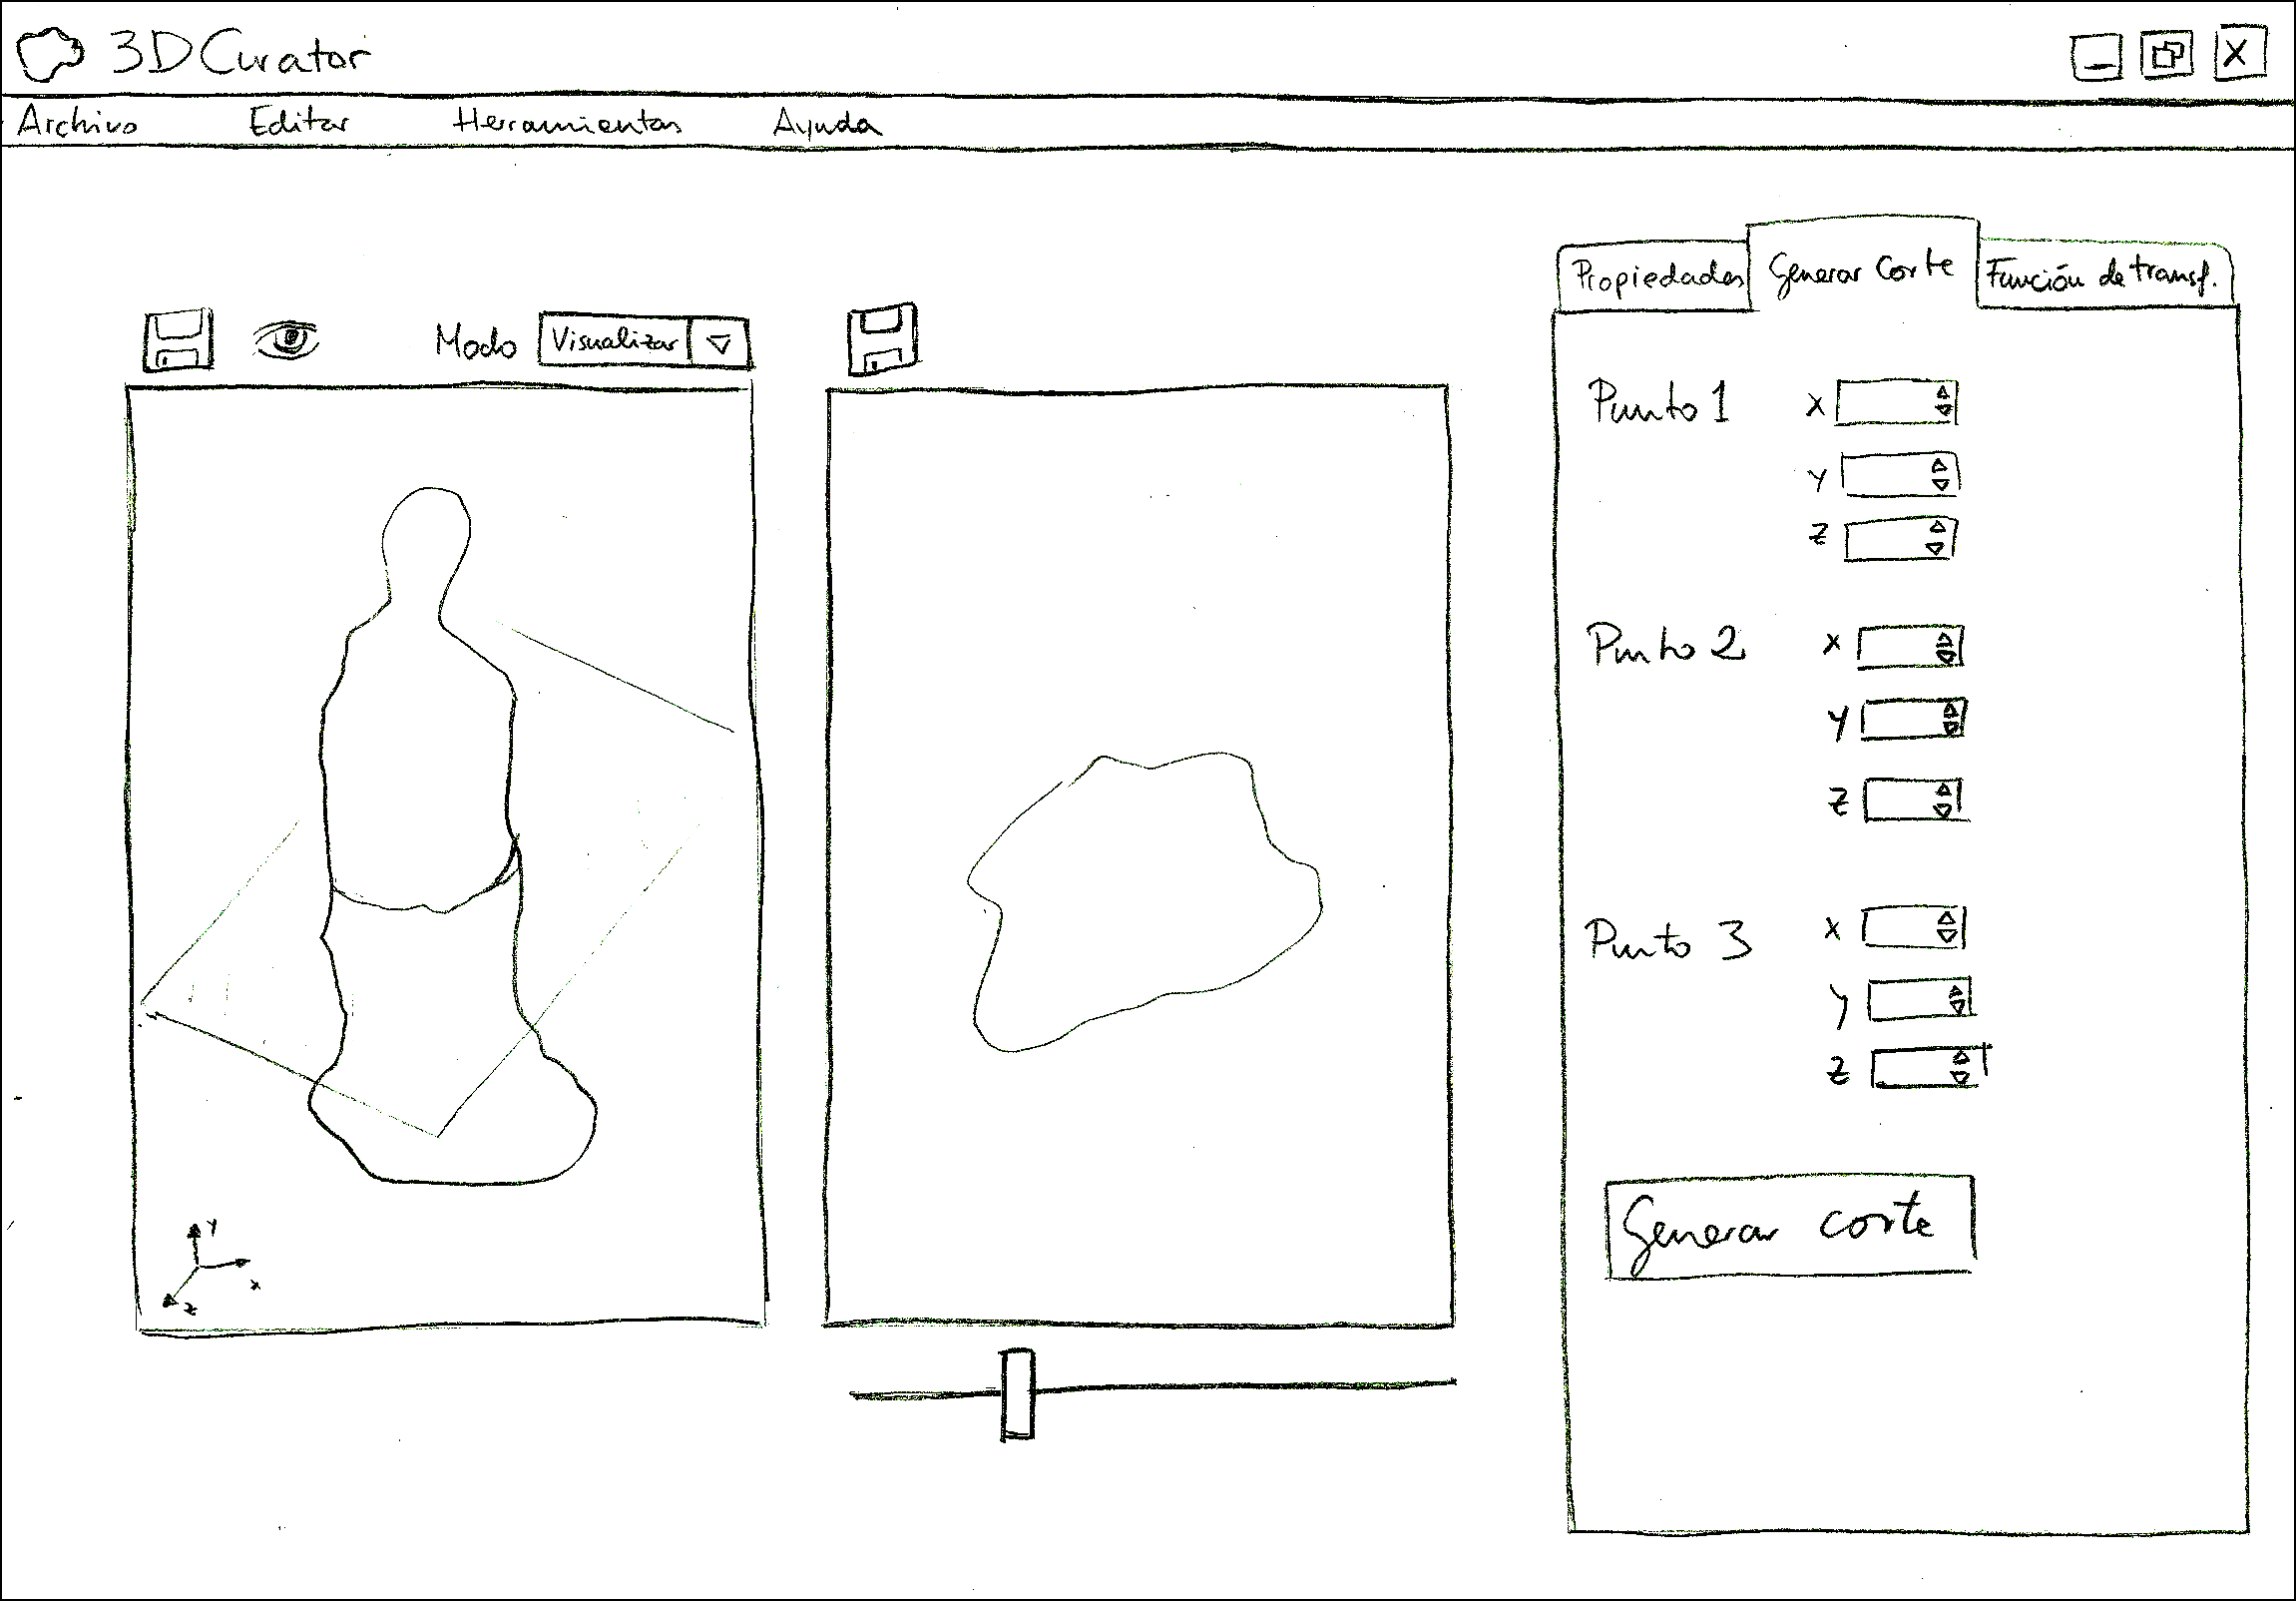
\includegraphics[width=12.5cm]{imagenes/basic_gui}
		\caption{Boceto a mano alzada de la posible distribución de los elementos en la GUI}
		\label{fig:basic_gui}
	\end{figure}
	
	\subsection{Funciones}
	
	El sistema tendrá que realizar distintas funciones que se comentaron anteriormente pero se profundizará en esta sección. Se han estructurado estas funciones por su objetivo separando cuatro subsecciones distintas: Lectura de datos, generación de cortes, visualización y configuración.
	
		\subsubsection{Lectura de datos}
		\begin{itemize}
			\item \textbf{Seleccionar carpeta}: Cuando el usuario quiera cargar datos DICOM, le aparecerá una ventana donde se podrá escoger alguna carpeta de su sistema de forma que solo muestre las carpetas y no los archivos.
			\item \textbf{Verificar que la carpeta contiene datos DICOM}: Se tendrá que verificar que el usuario ha seleccionado una carpeta con datos DICOM y se le avisará si no lo ha hecho.
			\item \textbf{Cargar datos DICOM}: Cuando se haya seleccionado una carpeta correcta, se cargarán los datos y automáticamente los visualizará en 3D con la configuración por defecto.
		\end{itemize}
	
		\subsubsection{Generación de cortes}
		\begin{itemize}
			\item \textbf{Definir plano}: El usuario podrá definir un plano por donde realizar un corte a la figura. Para ello tendrá que introducir tres puntos. Por defecto, se introducirá un plano en el eje XZ a una altura de Y = 0, siendo la dirección de los ejes XYZ la que utiliza VTK (Figura \ref{fig:vtk_axes}). El plano se podrá visualizar en el \textit{widget} de visualización 3D para ver gráficamente por dónde pasará.
			\begin{figure}[H]
				\centering
				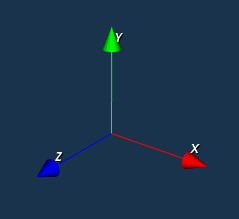
\includegraphics[width=8cm]{imagenes/vtk_axes}
				\caption{Dirección de los ejes XYZ}
				\label{fig:vtk_axes}
			\end{figure}
			\item \textbf{Modificar plano}: El usuario podrá modificar el plano o introduciendo nuevos puntos, o interactuando con la vista previa de éste en el \textit{widget} de visualización 3D. Las operaciones que podrá realizar en este serán:
			\begin{itemize}
				\item Rotar en cualquiera de los ejes.
				\item Trasladar en dirección de la normal.
			\end{itemize}
			\item \textbf{Generar corte}: Una vez se haya creado el plano deseado, se podrá mostrar el corte en el \textit{widget} de visualización de cortes.
		\end{itemize}
	
		\subsubsection{Visualización}
		\begin{itemize}
			\item \textbf{Visualizar en 3D}: Cuando el usuario haya seleccionado una carpeta con datos DICOM, se mostrará en 3D en el \textit{widget} izquierdo pudiendo rotar y hacer zoom interactuando con el ratón. Para visualizar el volumen se utilizarán técnicas de \textit{Direct Volume Rendering} que proporcionan VTK como puede ser el \textit{Ray-Casting}.
			\item \textbf{Visualizar corte}: Cuando el usuario haya cargado los datos DICOM y haya establecido un plano de corte, se podrá generar un corte a la figura por éste. Este corte se visualizará en el \textit{widget} derecho.
			\item \textbf{Guardar imagen}: El usuario en todo momento podrá guardar una imagen (en formatos comunes JPG o PNG) de lo que está viendo en cada uno de los \textit{widgets} seleccionando en una ventana que aparecerá cuando se elija la opción la dirección donde se guardará y el nombre del archivo. 
		\end{itemize}
	
		\subsubsection{Configuración}
		\begin{itemize}
			\item \textbf{Cambiar color de fondo}: El usuario podrá cambiar el color de fondo del \textit{widget} donde se mostrará la figura en 3D. Para ello podrá:
			\begin{itemize}
				\item Elegir entre colores predeterminados.
				\item Introducir un color mediante valores RGB.
				\item Introducir un color mediante su código de color hexadecimal.
			\end{itemize}
			\item \textbf{Cambiar función de transferencia}: El usuario podrá cambiar la función de transferencia utilizada para poder ver los distintos materiales con una paleta de color distinta a la que se da por defecto.
		\end{itemize}
	
	\subsection{Requisitos de rendimiento}
	
	Al ser una aplicación de escritorio donde no se almacenarán datos sino que se mostrarán, los requisitos de rendimiento no se centrarán en la concurrencia de acceso ni en el almacenamiento, como lo podrían estar en una aplicación web.
	
	Sin embargo, hay que tener en cuenta otros factores, como pueden ser el uso eficiente de memoria y no tener cargadas todas las figuras que se han estado visualizando, desechando la anterior cuando se carga una nueva.
	
	El rendimiento gráfico también es importante, por eso y para obtener imágenes de mayor calidad, se utilizarán técnicas de \textit{Direct Volume Rendering} como el \textit{Ray-Casting}. Estas técnicas necesitan una gran cantidad de procesamiento, pero la velocidad de procesamiento de las GPUs actuales no deberían resultar un problema.
	
	\subsection{Restricciones de diseño}
	
	Al utilizar la librería VTK se seguirá su estructura a la hora de construir el software, y se tendrán restricciones en cuanto a funcionalidad que se pueda construir con ésta. No obstante es una librería muy completa y no se debería encontrar ninguna restricción viendo otros programas de visualización de datos médicos que se han construido usando esta librería.
	
	\subsection{Atributos del software}
	
	Al usar CMake, se podrá crear un software multiplataforma que funcione en cualquier sistema operativo.
	
	El software generado deberá ser fiable, porque aunque no trabaje con datos sensibles cuya pérdida pueda ser grave, siempre resulta molesto utilizar un software con fallos que interrumpan durante su uso.
	
	También se debe tener en cuenta que el software sea mantenible pues, al ser libre, otros desarrolladores pueden colaborar en su desarrollo y debe estar bien documentado para que esto sea una tarea fácil.